\section{Design}

The Design of the test bed can be broken down into the following parts:

\begin{figure}
	\centering
	\includegraphics[scale=0.25]{ProtocolStack}
	\caption{An overview of the components of the system, including the OSI Layers they interact with.}
	\label{fig:ProtocolStack}
\end{figure}

\begin{itemize}
	\item USRP Software Defined Radio
	\item GNU Radio Flowgraph
	\item Batman-adv
	\item Flask Web Server
	\item SocketIO Web Sockets
	\item A.L.F.R.E.D. 
\end{itemize}

This configuration is shown in Figure \ref{fig:ProtocolStack}

\subsection{USRP Software Defined Radio}

For our project, we utilized a combination of Ettus Research USRP B200 and USRP B210 SDRs. These radios are able to communicate from 70 Mhz to 6 Ghz and are well supported in GNU Radio using the open-source USRP Hardware Driver (UHD) provided by Ettus. Their relatively low cost makes them ideal for building out larger testbeds. These serve as the radio transcievers for the current version of our platform. However, thanks to the UHD support in GNU Radio, any other USRP device will be compatible with the rest of the system, with little to no changes made to the development environment. 

\subsection{GNU Radio Flowgraph}

GNU Radio utilizes programs called ``Flowgraphs" to allow for graphical programming of of SDR software. To implement the physical and link layers on the SDR, we utilize the Out of Tree (OOT) module gr-mac created by John Malsbury \cite{0015}. This flowgraph is a very simplistic, but effective, implementation of a GMSK or OFDM transciever with a mac layer protocol called ``simple mac". There are two main blocks in the flowgraph. The first sets up the GMSK or OFDM radio. This heirarchical block is built by running a separate flowgraph which contains the UHD blocks to interface into the USRP as well as the modulation and demodulation blocks for the waveform. One of the more important aspects of the two Radio blocks, is that they convert from streaming data to message data. 

Most features of GNU Radio work on streaming data where there is constant data transmission in that portion of the flowgraph. However, packets are not sent continuously so separate logic is needed to convert streams to messages. These messages are passed into and out of the GMSK and OFDM heirarchical blocks, so the remainder of the flowgraph deals with passing messages only. 

We use the GMSK block to convert from streaming data to message data and then connect this block to a tunnel (TUN) or network tap (TAP) interface block. TUN/TAP devices are virtual network kernel devices supported entirely in software. TUNs are used to simulate layer 3 devices and TAPs simulate layer 2. Either of these could be selected to suit the users purpose, but as batman-adv is a layer 2 protocol, we will use the TAP protocol. This flowgraph also implements an 802.3 Tracker to build out a radio to address map of the network. 

\subsection{Batman-adv}

Batman-adv was chosen based on its large community and documented success as a mesh routing protocol \cite{5375690}. It is already included as part of the Linux Kernel, and additional software can be downloaded from most distributions repositories \cite{0008}. Configuring batman-adv to work on the SDR involves running the program batctl and selecting the recently generated TAP interface created by GNU Radio. The Maximum Transmission Unit (MTU) of the TAP interface must also be changed to 1532 from 1500 in order to incorporate the additional header batman-adv uses when sending data. With just Batman-adv and GNU Radio, we are able to create a Software Defined Radio based mesh network. The remainder of the test bed was implemented to leverage features unique to GNU Radio and Batman-adv to create a method of sharing frequency and other data in an effort to make cognitive radio testing much simplier. 

\subsection{Flask Web Server and Socket.IO}

\begin{figure}
	\centering
	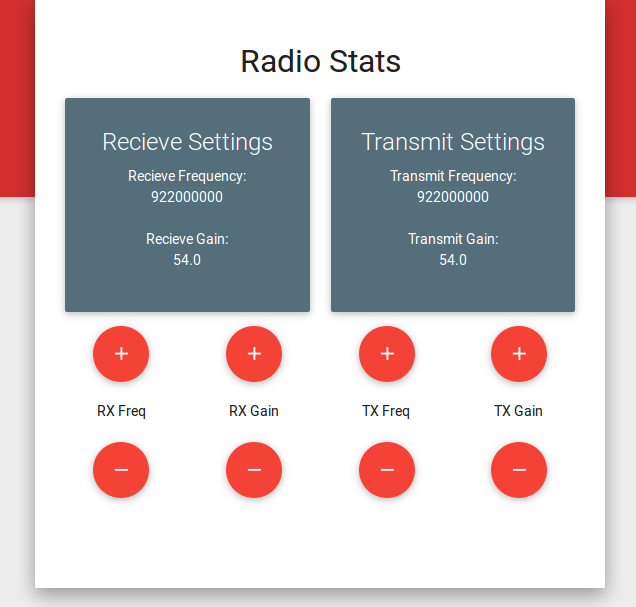
\includegraphics[scale=0.25]{WebInterFace}
	\caption{The web interface that lets the user initiate the network to hop to a new frequency.}
	\label{fig:WebInterface}
\end{figure}

Flask is a lightweight, open source, web framework for the Python programming language \cite{0011}. Flask was used to act as a broker between GNU Radio and any other user space applications or control systems we wished to implement. The Flask server runs the GNU Radio flowgraph in a background thread, while simultaneously configuring the TAP interface, setting up batman-adv, and starting A.L.F.R.E.D. as a background process. The only input needed from the user is an IP address for the TAP port, but this could later be replaced by running a DHCP server on the mesh network. 

Socket.IO is a javascript library that enables real-time bidirectional event-based communication \cite{0012}.  SocketIO was chosen as a means of relaying data between the flask server and other components of the system due to its speed, flexibility, and ability to broadcast messages to any connected client. Socket.IO also integrates easily into Flask \cite{0013} and can be used in stock python with a client library \cite{0014}. In flask, we create wrappers to all the necessary GNU Radio parameters so that external tools can relay data to and from GNU Radio over web sockets.  

We also use flask to host a single webpage that displays verious settings about the radio, and allows for the user to change parameters. The interface is shown in Figure \ref{fig:WebInterface} Since our platform does not yet include logic for automatic detection of primary users, we simulate this by allowing a person to click a button to change to a new frequency. This frequency will then be sent to the Flask server using web sockets. Flask recieves the request, and then uses A.L.F.R.E.D. to manage the next step. 

\subsection{A.L.F.R.E.D.}

 The ``Almighty Lightweight Fact Remote Exchange Daemon" or A.L.F.R.E.D. is a system for distributing data to all nodes on a mesh network \cite{0015}. A.L.F.R.E.D. is very simple to use, but still powerful. Whenver a node writes data to a channel on A.L.F.R.E.D., that data is passed from node to node to pass the data to all other members of the network. Typical uses for A.L.F.R.E.D. include keeping track of sensor data or building a visual map of the network. 

 An additional feature of A.L.F.R.E.D. is its ability to pass a command to the command line whenever new data is added. When the transmission frequency of the USRP is changed on the Flask server, Flask sends this information along with a UTC timestamp to A.L.F.R.E.D. before changing frequencies. A small delay is created so that we can be sure the information was sent to the other nodes before the node changes its broadcast frequency.  

 When the other nodes recieved the updated data table, A.L.F.R.E.D.'s callback function will run. This is a short program that parses the A.L.F.R.E.D. data table and looks for the most recent data it recieved. The callback function then sends the new frequency to Flask using Socket.IO which causes Flask to change the frequency in the GNU Radio flowgraph.   